%%%%%%%%%%%%%%%%%%%%%%%%%%%%%%%%%%%%%%%%%%%%%%%%%%%%%%%%%%%%
% pakete einbinden
\documentclass[11pt,oneside,headsepline,footsepline]{scrreprt}
\usepackage[latin1]{inputenc}           % f�r Umlaute
%\usepackage{a4}                         % A4-Format
\usepackage{geometry}
\geometry{a4paper,body={5.8in,9in}}
%\usepackage{layouts}                    % Seitenlayout mit anzeigen
%\usepackage{latexsym}                   % besondere Symbole
\usepackage{amsfonts, amsmath, amssymb, amsthm} % AMS Mathematik Packete
%\usepackage{calc}                      % Rechnen mit LaTex Werten
\usepackage{booktabs}                   % f�r sch�nere Tabellen
\usepackage{fancybox}                   % Gleichungen einrahmen
%\usepackage{fancyheadings}
\usepackage{fancyhdr}                   %fancyhdr: Paket f�r Kopf- und Fusszeilen-Formatierung 
\usepackage{multicol}
%\usepackage{float}                      % Flie�umgebungen festlegen k�nnen
%\usepackage[section]{placeins}          % Ermoeglich \Floatbarrier fuer Gleitobj. an Abschnittsgrenzen
\usepackage{graphicx}                   % Grafiken einbinden
\usepackage[hang]{subfigure}            % Teilabbildungen erstellen
\usepackage{calc}                       % Rechnen m�glich
\usepackage{listings}                   % schoene Quellcodes
%\lstloadlanguages{C}                    % Listings standardsprache setzen
\usepackage{url,xspace,boxedminipage}   % stelle URL's ordentlich dar
%\usepackage[thickspace]{SIunits}        % physikal. Einheiten
\usepackage{acronym}                    % fuer Acronyme
\usepackage{color}                      % zur eigenen Farbdefinition mit \definecolor
\usepackage{nicefrac}                   % Sch�ne Br�che im Flie�text
%\usepackage{ngerman} 
% -------------------------------------------------------------------------
%\usepackage[T1]{fontenc}	%T1, fontenc: Worte mit � richtig schreiben
%??% \usepackage{longtable}		%longtable: �berlange Tabellen automatisch umbrechen
%??% \usepackage{array}		%array: erweitertes Paket f�r die Umgebung array, tabular und tabular*
%??% \usepackage[small,bf]{caption}	 %caption: kleinere Schriftgr�sse f�r die Bildbeschreibung
%??% \usepackage{cite}		%cite: Literaturverweise z.B. 1,2,3 werden zusammengefasst: 1-3
%??% \usepackage{makeidx}
%??% \usepackage{float}      % Stellt die Option [ht] fuer Floats zur Verfgung 
%??% \usepackage[pdftex,urlcolor=blue,linkcolor=black,a4paper,colorlinks=true]{hyperref}


\lstset{ %
%language=C++,                % choose the language of the code
%basicstyle=\scriptsize\ttfamily,       % the size of the fonts that are used for the code
%numbers=left,                   % where to put the line-numbers
%numberstyle=\footnotesize,      % the size of the fonts that are used for the line-numbers
%stepnumber=1,                   % the step between two line-numbers. If it is 1 each line will be numbered
%numbersep=5pt,                  % how far the line-numbers are from the code
backgroundcolor=\color{white},  % choose the background color. You must add \usepackage{color}
showspaces=false,               % show spaces adding particular underscores
showstringspaces=false,         % underline spaces within strings
showtabs=false,                 % show tabs within strings adding particular underscores
frame=tb,                   % adds a frame around the code
tabsize=3,              % sets default tabsize to 2 spaces
captionpos=b,                   % sets the caption-position to bottom
breaklines=true,        % sets automatic line breaking
breakatwhitespace=false,    % sets if automatic breaks should only happen at whitespace
mathescape=true,						% sets if latex math environment will be honored ($...$)
escapeinside={(*@}{@*)}     % if you want to add a comment within your code
%escapeinside={\%}{)}   
}


\ifx\pdftexversion\undefined
\usepackage{hyperref}
\else
\usepackage[colorlinks=false,       %true => text des links wird farbig, false => farbiges kaestchen (wird nicht gedruckt) um schwarzen text
            linkcolor=black,        %nur bei colorlinks=true
            urlcolor=black,
            citecolor=black,
            bookmarks,                  % Bookmarks erstellen
            bookmarksopen=true,         % Bookmark beim Oeffnen anzeigen?
            pdfpagemode=UseOutlines,    % Bookmark beim Oeffnenanzeigen? (UseOutlines / none)
            bookmarksopenlevel=3,       % bis zu welcher Ebenen geoeffnet
            bookmarksnumbered,          % Kapitelnummern in Bookmarks
            %pdfkeywords={a,b},
            ]{hyperref}
\fi
\usepackage[figure]{hypcap} % Links auf Gleitumgebungen springen nicht zur Beschriftung, sondern zum Anfang der Gleitumgebung 

%%%%%%%%%%%%%%%%%%%%%%%%%%%%%%%%%%%%%%%%%%%%%%%%%%%%%%%%%%%%%
% definitionen:
\ifx\pdftexversion\undefined
\else
\pdfoutput=1        % PDF-Ausgabe anschalten.
\pdfimageresolution=600
\pdfcompresslevel=9 % 0 keine kompression, 9 staerkste kompression
\fi

\DeclareGraphicsExtensions{.pdf,.png,.jpg,.eps}
\graphicspath{{./fig/}} %alle Bilder werden in diesem Unterverzeichnis gesucht

%trenntabelle
\hyphenation{whe-ther}

% schoene kopf-fusszeilen
\pagestyle{headings}

% ungenaue silbentrennung
%\sloppy

%\pagestyle{fancy}

%Eigene Kommandos
\newcommand{\cu}[0]{computing unit}
\newcommand{\cus}[0]{computing units}


\newcommand{\functionname}[1]{\textit{#1}}
\newcommand{\codesnippet}[1]{\textit{#1}}
\newcommand{\cdefine}[1]{\verb�#1�}
\newcommand{\consolecmd}[1]{\verb�#1�}

\makeatletter
\newcommand{\todo}[1]{%
	\pdfstringdef\@tempa{#1}%
	\marginpar{%
	\leavevmode%
	\pdfannot  width  12cm  height  \baselineskip  depth  0pt{
		/Subtype  /Text
		/Contents  (ToDo: \@tempa)
		}%
	}%
	\let\@tempa\relax%
}%
\makeatother

%\renewcommand{\todo}[1]{} %Todo auslassen

\begin{document}


\title{Kernel-Space Scheduler \\ User Guide \\[1cm] \large{Version 1.0}}
\author{Tobias~Wiersema, Tobias~Beisel} 
\maketitle

%roemische seitenzahlen
\pagenumbering{roman}
\renewcommand{\headheight}{14.5pt}

% Setzen des bibliographischen Stils. Insbesondere empfehle ich
% fuer advanced usage die Benutzung von natbib, hier aber der
% Einfachheit nicht eingebunden

%\bibliographystyle{plain}
\bibliographystyle{alpha}


\thispagestyle{empty}

%%%%%%%%%%%%%%%%%%%%%%%%%%%%
% Deckblatt-Format:
%chapter und sections nicht in grossschrift im header ausgeben
\renewcommand{\chaptermark}[1]{\markboth{\chaptername \ \thechapter.\ #1}{}}
\renewcommand{\sectionmark}[1]{\markright{\thesection.\ #1}}



\cleardoublepage
%%%%%%%%%%%%%%%%%%%%%%%%%%%%
%\setcounter{tocdepth}{1} % tiefe des inhaltsverzeichnisses
\tableofcontents
\cleardoublepage
\listoffigures
\cleardoublepage
%\listoftables
%\cleardoublepage
\lstlistoflistings
\cleardoublepage

%\lstlistoflistings
%\cleardoublepage

%%%%%%%%%%%%%%%%%%%%%%%%%%%%
\pagenumbering{arabic} 
%%%%%%%%%%%%%%%%%%%%%%%%%%%%%%%%%%%%%%%%%%%%%%%%%%%%%%%%%%%%%%%%%%%%%%%%%%%%%%%%%%%
\chapter{Testapp manual}
\label{Testapp}

Testapp is an application framework designed to simplify the employment of the programming model needed to make use of the time-shared kernel extension. If you are unfamiliar with this application model, see section \ref{Concept:APM} for details on it.

Testapp should enable programmers to meet all requirements to work with the scheduler extension, without reimplementing the global program flow for every application. It therefore implements the program flow depicted in figure \ref{fig:FlowDiaHWT} in an easily extensible manner, thereby enforcing the use of cooperative multitasking. Section \ref{Implementation:Userside} describes the framework and two exemplary implementations, which make use of it.

Section \ref{Porting} then describes the steps necessary to port an existing application to this APM.

How a vanilla Linux kernel can be extended with the new accelerator scheduler is explained in section \ref{ExtendKernel}.


\section{Application programming model}
\label{Concept}
\label{Concept:APM}

Applications are required to implement a specific programming model in order to make full use of the accelerator scheduling kernel extension. We made this design choice since the scheduler needs a method to pass the control of a processing unit to a specific task, but the NVIDIA CUDA runtime so far only provides a first-come-first-serve scheduler. As the CUDA libraries are closed source, the only way to ensure that only a scheduled task is allowed to execute would be a library wrapper for them. This wrapper would have to communicate with the CUDA libraries and could hence not be fully integrated into the kernel. A daemon in user space would be necessary since it additionally would have to react to the scheduling decisions of the extension. As the user space side was only of interest for evaluation purposes and not the focal point of this approach, we decided against the user space daemon in favor of a more simple but still effective programming model which employs cooperative multitasking. This model will be detailed in the remainder of this section.

As threads are our schedulable entities they also are the scope of our model. Chapter~\ref{Implementation} will give an overview over one possible integration of this concept into a complete application. Applying the model to a thread creates a task which communicates with the scheduler extension, allowing the operating system to administer the usage of its heterogeneous \cus{}. We will call such a task a ``hardware task'' in this document. It has to provide an implementation of its main algorithm for one or more architectures in the corresponding binary format and has to invoke the code designed for the unit which the extension assigns to it. Every actual communication with the devices themselves has to be done by this task, since the libraries needed to perform that communication are at least in the case of NVIDIA GPUs closed source user space libraries. We call the administrative part of the hardware task its ``ghost thread''. If the scheduler assigns a CPU core to a hardware task, the differentiation between the computational part and the ghost thread is merely of organizational nature, as both parts will mostly be performed by the same thread. In the case of hardware accelerators however the ghost thread is the part which has to be run on a CPU, i.e. the part that executes the system calls, branches to the correct device code, performs the memory management and copies the data to and from the device, invokes the computational part on the accelerator and waits for its completion. The name ``ghost thread'' stems from this list of activities, as it is a shadow representative of the accelerator code, which the scheduler can manipulate and schedule. It does not stress the CPU on which it is executed, because it primarily carries out blocking I/O functions, and thus waits most of the time.

An existing application can source out every part that is acceleratable to a hardware task. This is not limited to parallel computations, since the ghost threads are standard POSIX threads, and hence the program may wait for them to finish before proceeding, or synchronize with them in any other standard way. If it provides CPU and NVIDIA CUDA implementations, a program augmented with hardware tasks would be able to run on a system with or without a CUDA card, without change to the program. Two such programs could run in a system with one card using an interleaving execution pattern on the unit, orchestrated by the scheduler extension. This time sharing would allow for continuous accessibility of the accelerator from the users point of view, and could increase the possible interactivity of both programs.

Figure~\ref{fig:FlowDiaHWT} displays the program flow of a hardware task. The steps in which data or code is copied or such resources are released, only apply to accelerators and may be skipped for execution on a CPU. Analogously, while the ghost threads actually wait in a blocked state for the accelerator to reach the next checkpoint, they have to perform the calculation steps to reach that checkpoint if the assigned unit is a CPU.
\begin{figure}[htbp]
  \centering
    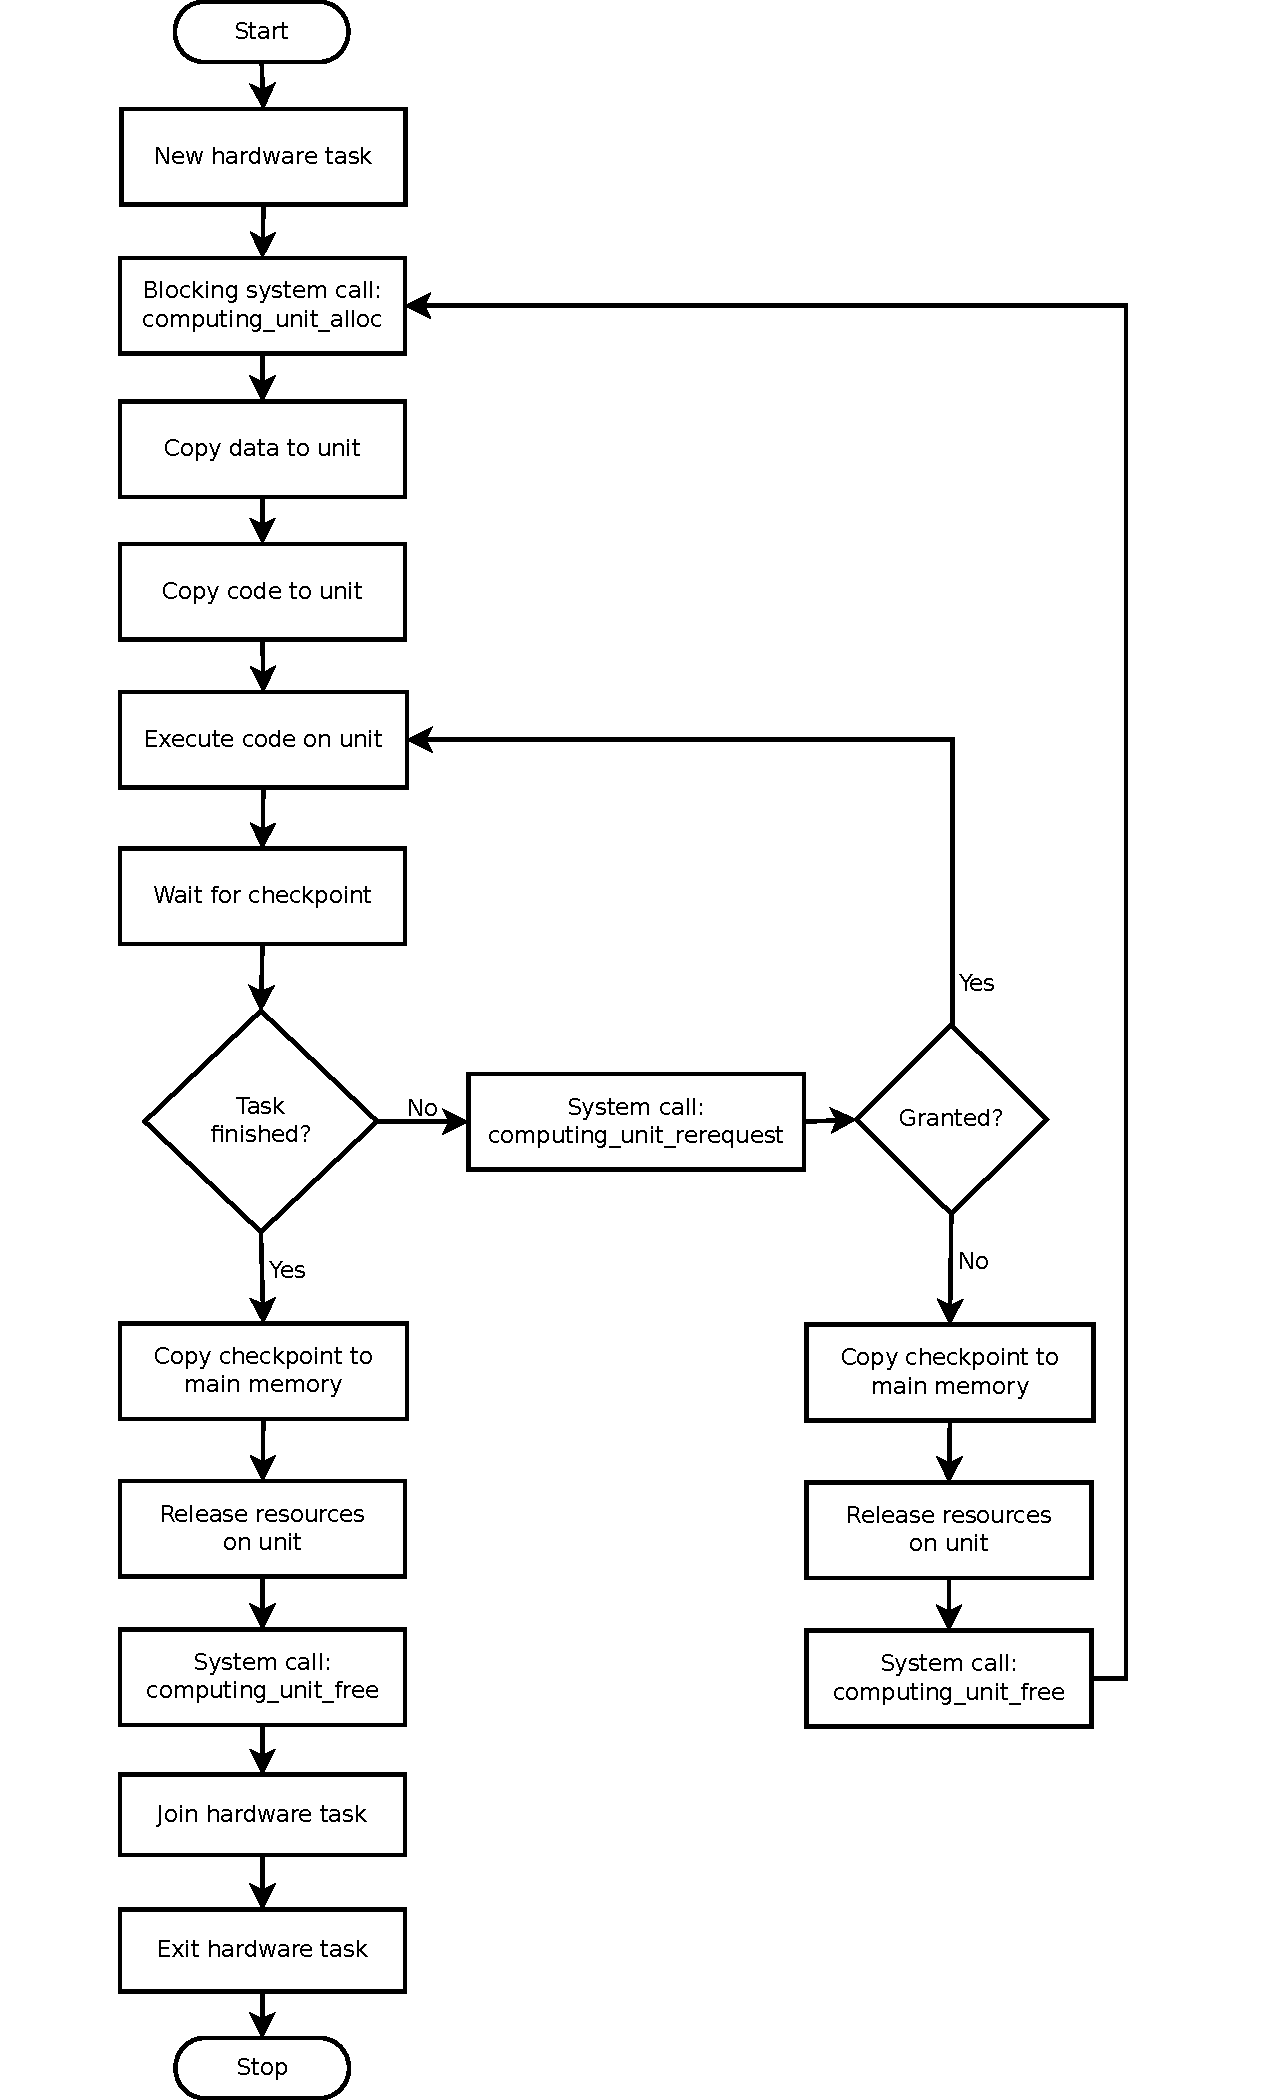
\includegraphics[width=0.90\textwidth]{FD_hardware_task}
  \caption[Program flow of a Hardware Task]{Program flow of a hardware task.}
  \label{fig:FlowDiaHWT}
\end{figure}
After being created by its parent task, a hardware task has to allocate a \cu{} using the \functionname{allocation} system call of the scheduler extension. This call blocks until a valid resource could be found or fails if there are no suitable devices present in the system. Should the call return, the hardware task may allocate memory on the assigned device and copy its data to it. This may be a checkpoint from a previous run or just constant or initial data. Afterwards it should copy the binary with the device code to the resource and start the execution. If the assigned unit is a CPU then the hardware task actually performs the computation itself here, or it starts a delegate thread for that purpose. If either a new checkpoint has been reached or the task has finished all calculations, the execution returns. If the task has not finished its work and can continue to use the last assigned accelerator, it should re-request the unit from the kernel extension, as all needed computing resources are still on it. The scheduler may then grant or deny that request. Should it allow the further occupation of the unit, the task executes the code again to advance to the next checkpoint (or the end). If either the re-request has been denied or if the task has reached the last checkpoint, the hardware task has to copy the current checkpoint from the resource to main memory. Afterwards all allocated memory regions on the device have to be released. To signal the scheduler that it completely left the device, it then has to call the \functionname{free} routine of the extension. In case of a denied re-request the task can afterwards invoke the \functionname{allocation} call again, to request access to the same or another resource. If the task was done, it can be joined in the parent thread before exiting, using conventional threading methods.

The application may only copy data from or to and execute on a device which has been assigned to it via the \functionname{computing\_unit\_alloc} call. The assignment mechanism can therefore be seen as a locking technique not unlike a semaphore, where a hardware task has exclusive access to a computing unit between the system calls \functionname{computing\_unit\_alloc} and \functionname{computing\_unit\_free}.

There are two new structures defined in the kernel extension, which are needed for the \functionname{allocation} system call. They are defined in a public header file that can be embedded in applications.
The first of them is \codesnippet{struct meta\_info} and is defined as shown in Listing~\ref{lst:meta_info}, which has been reduced to key components. The field \codesnippet{memory\_to\_copy} denotes the amount of memory which has to be transferred to and from the device, and will obviously not be considered if the task is currently working on a CPU, as the checkpoint does not need to be copied in that case. Using this information together with the bandwidth of the device, the scheduler can estimate the time it will take to perform a task switch to or from this task. Hence this value is integrated into the individual scheduling granularity for this task. The \codesnippet{parallel\_efficiency\_gain} has to be estimated by the software developer on an arbitrary scale from $0$ to $5$. It should roughly reflect how much the application will benefit if it can be scheduled on a device that is capable of data-parallel computation. Values of $0$ and $1$ will lower the affinity of this task towards such \cus{} and at the same time raise the affinity towards sequential units. Values of $4$ and $5$ influence the affinities analogously, with interchanged roles. A value of $2$ is neutral and as such has no impact on the affinities. \codesnippet{type\_affinity} is an array which is holding the affinity of the application towards the different \cu{} types that the kernel knows of. An affinity value of zero has a special meaning, as it indicates that no algorithm implementation is available in the application for that unit type. Other than that higher values correspond to higher affinity, i.e. tasks prefer the units to which they have higher affinity values.  Application programmers can use this field to encode information about the efficiency of the algorithm implementations, or just as indicator which implementations are given and which are not. Obviously the ability to parallelize the problem should not be included in this estimation unless \codesnippet{parallel\_efficiency\_gain} has been disabled using the neutral value of $2$. The calling application is free to calculate the gain or base affinity dynamically from its inputs, as the structure is a parameter of the \functionname{allocation} call and can thus be altered between different invocations thereof.

\begin{lstlisting} [float=htbp,caption={Shortened meta information data structure}, label={lst:meta_info}, language=C++]
struct meta_info {
	//In MB. The amount of memory which has to be transferred to and from the device.
	unsigned int memory_to_copy;
	
	// How much the task benefits from data-parallel execution on a scale from 0 (not parallelizable or small problem scale; no speedup expected from parallelization) to 5 (completely parallelizable large scale problem).
	int parallel_efficiency_gain;
	
	// Affinity of the task towards the different unit types. Valid range: [0-15]
	unsigned int type_affinity[CU_NUMOF_TYPES];
};
\end{lstlisting}

The second data structure is \codesnippet{struct computing\_unit\_shortinfo}, which can be found in Listing~\ref{lst:cu_shortinfo}. This structure is a data container, designed to include every bit of information that user space applications typically need to work with the scheduler and the assigned devices.
The basic information about the unit which an instance of this structure currently represents, is given by a unique \codesnippet{handle} that corresponds to a unit's id and by its \codesnippet{type}, encoded as integer with constants that are defined in the same header file. The \codesnippet{api\_device\_number} holds the number with which the device can be identified in its own API, thus enabling the calling application to use the correct accelerator. For NVIDIA CUDA devices this would be the numeric parameter which has to be passed to the \codesnippet{cudaSetDevice} call. As user space applications may display or process information about current statistics of the unit, the kernel provides the three last fields of the structure. \codesnippet{count} denotes the number of currently executing tasks on that device, while \codesnippet{waiting} holds the number of tasks that are waiting in the red-black-tree. The field \codesnippet{online} indicates if this device is currently being used by the scheduler extension or not. Offline units do not accept tasks and are therefore irrelevant for the \functionname{allocation} system call.

\begin{lstlisting} [float=htpb,caption={[Communication data structure between kernel and user space]computing\_unit\_shortinfo data structure}, label={lst:cu_shortinfo}, language=C++]
struct computing_unit_shortinfo {
	unsigned long handle;
	unsigned int type;
	unsigned long api_device_number;
	int count;
	int waiting;
	int online;
};
\end{lstlisting}

The application has to call \functionname{computing\_unit\_rerequest} periodically to ask for permission of the scheduler to occupy the unit further. Before calling, the program should have reached a point of execution where it is possible to leave the \cu{}, since the scheduler could deny the re-request. As mentioned before, we call such an application state a ``checkpoint''. At such a point, the application has to make sure that it can extract the complete state information from the unit, for instance by saving it into accessible device memory. If the scheduler then denies the re-request, this checkpoint has to be copied to the main memory by the ghost thread. After releasing all resources on the device the ghost thread thirdly has to call \functionname{computing\_unit\_free} to inform the scheduler of the availability of the unit. If the hardware task is not done at this point, it may call \functionname{computing\_unit\_alloc} again to get a \cu{} on which it can continue the calculation, as depicted in figure \ref{fig:FlowDiaHWT}.


\section{Exemplary test applications}
\label{Implementation}
	\label{Implementation:Userside}
To obtain performance evaluations of the scheduler extension concept and its Linux kernel implementation, we implemented exemplary applications that employ the programming model described in Section~\ref{Concept:APM}. They are embedded into a framework which consists of a general management part and an abstract base class that aims to enforce the use of cooperative multitasking and which should be extended by problem specific threads.

The following subsection will detail the framework, which can be used to rapidly generate new test applications. Subsections \ref{Implementation:Userside:MD5} and \ref{Implementation:Userside:PF} introduce approaches to solve two exemplary problems using hardware tasks and the framework.

\subsection{Framework}
\label{Implementation:Userside:Framework}
The goal of the framework presented in this section is to provide a set of C++ classes that ease the use of the new system calls while making an effort to force deriving classes to employ the cooperative multitasking scheme.

The main purpose of the application framework is to provide feasible methods for the execution of hardware tasks which may be able to operate on more than one \cu{} type, and that should employ checkpointing to enable cooperative multitasking. It therefore contains no problem specific code, but an abstract base class \codesnippet{Worker} that already makes use of the new system calls in a reasonable fashion. Once finished with a deriving subclass that overwrites all pure virtual methods of class \codesnippet{Worker}, and provides a set of algorithm implementations for different \cus{}, the result is a complete application which makes full use of accelerated hardware tasks.

When started, such an application creates one or more instances of the available \codesnippet{Worker} class implementations, waits for their completion, and joins and destroys them afterwards.

The abstract base class already includes a main loop, which employs the program flow introduced in Figure~\ref{fig:FlowDiaHWT}. Upon creation, it generates the meta information from the current problem parameters by calling the pure virtual function \functionname{workerMetaInfo}. The affinities calculated therein also have to reflect the algorithm implementations which the subclass provides, by assigning an affinity of zero to every unsupported \cu{} type. Using the generated data, the scheduler is able to find the most suited device for this task in the \functionname{allocation} routine, which the application calls afterwards. To use the returned device, it has to be initialized with the latest checkpoint or the initial parameters and allocated working memory. Then the binary has to be started as often as necessary for the deriving class and allowed by the \functionname{re-request} system calls. Afterwards, the resulting checkpoint has to be downloaded again and all memory freed on the device, prior to calling the \functionname{free} system call of the kernel extension. Thus, the \codesnippet{Worker} class expects three functions in the subclass, to handle the assigned unit type. An \functionname{initialization} routine, a \functionname{main} execution and a \functionname{free} function. The application determines these functions by passing the assigned unit type to the pure virtual function \functionname{getImplementationFor}, which has to return three function pointers.

The \functionname{initialization} function will be called after the successful return of the \functionname{allocation} system call. It should allocate memory on the assigned device and copy the latest checkpoint into it. The communication with the device should be performed using its native libraries. If possible, this function should also copy the code to the unit.

The purpose of the \functionname{main} execution function is to copy the code and parameters to the device if necessary, to start the computation and to wait for it to finish. The execution unit on the device then calculates the next checkpoint from the last one. With the checkpoint ready in device memory, the \codesnippet{Worker} class calls the \functionname{re-request} routine of the scheduler extension, to determine whether or not it has to leave the \cu{}. It loops the call to the \functionname{main} execution routine as long as the re-requests succeed and there is still work to do.

If a re-request fails, or if the application is done, it calls the \functionname{free} routine of the subclass, which copies the checkpoint from device memory to main memory and then releases all memory regions currently held by the application on the device. To inform the scheduler that it has finished this computation it then calls the \functionname{free} function of the kernel extension.

Depending on the state of the problem solving part of the subclass, the \codesnippet{Worker} object either exits at this point, or loops to the \functionname{allocation} call, if there is still work left to be done.

This concludes the description of the framework. A subclass has to provide the following items to complete the framework to a working application:
\begin{enumerate}
	\item An implementation for the pure virtual function \functionname{workerMetaInfo}, which calculates the contents of the \codesnippet{meta\_info} structure from the problem parameters and available algorithm implementations
	\item A triplet of functions per supported device type that perform the following actions:
	\begin{itemize}
		\item Initialization of the \cu{}
		\item Execution of the code on the unit
		\item Freeing of the resources allocated by the two above functions
	\end{itemize}
	\item An implementation for the pure virtual function \functionname{getImplementationFor}, which returns the triplet of functions that implement the algorithm for the given unit type
	\item A unit specific implementation of the algorithm, which then is executed on the device by the execution routine
\end{enumerate}

For the implemented exemplary implementations, the possible unit types were CPU or NVIDIA CUDA GPU. For the CPU case, the \functionname{initialization} and \functionname{free} functions of the subclasses are dummy functions, as in this case the checkpoints are already in the main memory and hence do not have to be allocated or copied.

\subsection{MD5 Cracking}
	\label{Implementation:Userside:MD5}
MD5 is the name of a hashing function developed by Ron Rivest in 1992 \cite{rivest1992md5}. Its use in secure applications is discouraged nowadays, as several flaws of the algorithm have been discovered which result in security weaknesses. Researchers found ways to generate MD5 collisions (e.g. \cite{stevens2009cpc}), i.e. situations in which two different inputs yield the same MD5 hash. The exemplary application presented in this section implements a brute force attack, the most naive approach to reverse the hash function. We chose this approach because it uses only the well-known MD5 algorithm and is computationally intensive with long running times, which makes it a good candidate to test and evaluate a scheduler.
	
The implemented attack is based on the knowledge of the input string's length and the alphabet, i.e. the list of possible characters used in the string. Given the MD5 hash and length of a target string the application checks the MD5 hashes of all possible combinations of characters from the alphabet that are of the same length. If one of that combinations yields the same MD5 hash as the input string then that combination is assumed to be the target string. As the inspection of one possible solution is completely independent from that of the others, and as the algorithm applies the same instructions to a large set of data, this application benefits greatly from data-parallel SIMD computation.

In more mathematical terms, the problem is defined as follows:\\ Given an alphabet $\Sigma$ as set of characters, the input $h$ to the main algorithm is the MD5 hash of a string $t$ of length $n$ over the alphabet $\Sigma$. Repetitions of characters in $t$ are allowed. In other words: $h = \text{md5}(t)$ with $t \in \Sigma^{n}$. The search space of the algorithm consists of all combinations of characters from $\Sigma$ and hence is limited ($|\Sigma^{n}| = |\Sigma|^{n} < \infty$) and can be enumerated and thoroughly searched in finite time. The cracking routine makes use of such an enumeration as Listing~\ref{lst:MD5Cracking} shows. The enumeration itself is irrelevant for the description of the algorithm, but it is crucial that all provided implementations use the same enumeration of the search space. This allows the application to use the number of the last inspected word as checkpoint, because it contains all the information that is needed to describe the complete running state of the program: ``Every word up to the $i$th has been checked and none of them has been the target word''. That none of the words below $i$ can be the target word is implicated by the existence of the checkpoint. If the target word would have already been found, the program would have exited and hence there would be no checkpoint.

\begin{lstlisting} [float=ht,caption={MD5 cracking using a brute force attack}, label={lst:MD5Cracking}, language=C++, morekeywords={for,let}]
md5_crack($h$, $\Sigma$, $n$){
	// enumerate all possible words
	for $i$ from $1$ to $|\Sigma|^{n}$ do
		// generate the $i$th word
		let $w$ be the $i$th word in $\Sigma^{n}$
		// compare its MD5 hash to the target
		if md5($w$) == $h$
			return $w$   // return successfully if they match
	done
}
\end{lstlisting} 

To make use of all aspects of the managed acceleration provided by the scheduler extension, the algorithm has to be implemented for different \cus{}. Our exemplary implementation includes hardware tasks that can use either CPUs or NVIDIA GPUs for computation. The concept of the core algorithm is realized in both versions, though only the CPU version follows the strictly sequential flow presented in Listing~\ref{lst:MD5Cracking}. Theoretically the algorithm reaches a new possible checkpoint at every iteration of the loop. Invoking the \functionname{re-request} system call that often would introduce a large scheduling overhead though, and thus the application calls it only every few hundred iterations. The CUDA implementation exploits the independence of the hash calculation for the different character combinations. It inspects a batch of words in parallel in each iteration, starting from the last checkpoint. The size of the batches is a tunable parameter in the implementation. On our test system a batch size of one million hashes at once\footnote{The complete batch is not necessarily executed in parallel, but the CUDA GPU has a scheduler of its own that strives to run as many CUDA threads in parallel as possible. This refers to the scheduler on the accelerator, not to the first-come-first-serve scheduler implemented in the driver.} still produced good results.

Since the scheduler has the choice to schedule the application on a GPU or on a CPU it needs additional information to learn which unit it shall prefer. Therefore the hardware task of the program has to include meta information about itself in the call to the scheduler's \functionname{allocation} routine. In our implementation of the kernel extension concept this information contains the size of a checkpoint, the size of the memory that has to be allocated on the device for the calculations, how much the task gains from data-parallel execution and an affinity map towards the possible \cu{} types. Since most of this data varies at runtime, the kernel extension only expects estimates that provide enough information to make a reasonable decision.

For MD5 cracking the routine to estimate the meta information works as shown in Listing~\ref{lst:MD5metainfo}. It sets \codesnippet{memory\_to\_copy} to zero, as a checkpoint for this application consists of just one number, and hence its size is negligible if measured in megabyte. The estimated \codesnippet{parallel\_efficiency\_gain} of data-parallel execution depends to a degree on the overall size of the search space $\Sigma^{n}$.

\begin{lstlisting} [float=ht,caption={[Meta information for MD5 Cracking]Procedure that generates the meta information for MD5 cracking}, label={lst:MD5metainfo}, language=C++, morekeywords={uint64}]
workerMetaInfo(struct meta_info *mi)
{
	mi->memory_to_copy := 0 // Checkpoint size in MB
	
	// guess efficiency gain from number of possible character combinations
	switch ($|\Sigma^{n}|$)
	case $|\Sigma^{n}|$ <= 10000
		mi->parallel_efficiency_gain := 0
	case $|\Sigma^{n}|$ <= 100000
		mi->parallel_efficiency_gain := 1
	case $|\Sigma^{n}|$ <= 200000
		mi->parallel_efficiency_gain := 2
	case $|\Sigma^{n}|$ <= 500000
		mi->parallel_efficiency_gain := 3
	case $|\Sigma^{n}|$ <= 1000000
		mi->parallel_efficiency_gain := 4
	case else
		mi->parallel_efficiency_gain := 5
	
	// more affine to GPU
	mi->type_affinity[CU_TYPE_CUDA] := 2
	mi->type_affinity[CU_TYPE_CPU] := 1
}
\end{lstlisting} 

If the search space contains only a few thousand possibilities, then the overhead of starting a computation on a device capable of running the algorithm data-parallel outweighs the benefits. Hence, the data-parallelism is estimated to have little or negative impact for small problem sizes, while providing faster speeds for search spaces that span hundreds of thousands of candidates. As this exemplary application provides implementations for two different architectures its affinity map contains two entries greater than zero. One for the unit type CPU and one for the type CUDA GPU. We set the affinity towards GPUs twice as high as that towards CPUs, since the application is generally better fitted to run on a GPU than on a CPU, because it has to copy only a small amount of code and data to the device and because of its parallelizable nature.

\subsection{Prime factorization}
	\label{Implementation:Userside:PF}

Prime factorization denotes the problem of factorizing a number into its prime factors. This factorization is unique except for the order of the factors. This example application calculates the factorization by trying all possible factors in successive order. While this may seem to be a naive approach, it can indeed be optimized in a few ways that result in a fast algorithm.

Listing~\ref{lst:PFCPU} shows most of the optimizations that we applied. The algorithm returns the factorization as two arrays. F contains the prime factors and M their respective multiplicity. To decrease the runtime it only searches for factors up to the square root of the target number. If the algorithm finds a factor, it reduces the target number by that factor as often as possible, thereby determining the multiplicity of it.

\begin{lstlisting} [float=ht,caption={Prime factorization algorithm}, label={lst:PFCPU}, language=C++, morekeywords={end,then,done}]
pf($a$){
	// initialize the return arrays
	F := $\emptyset$
	M := $\emptyset$
	$c$ := $a$ // start with the provided number
	// loop from first prime up to square root of current number
	for $i$ from $2$ to $\sqrt{c}$ do
		if $c$ == 1 then break  // factorization complete
		if $c$ mod $i$ == 0
			F := F $\cup$ $i$ // add factor to F
			M[$i$] := 0 // determine the multiplicity of it
			while $c$ mod $i$ == 0
				$c$ /= $i$ // update the target number accordingly
				M[$i$] += 1
			end while
		end if
	done
	
	// if the number is not $1$ the factorization is not complete, but as no additional factor has been found the remainder must be prime itself
	if $c$ > 1
		F := F $\cup$ $c$
		M[$c$] := 1
	end if
	
	return F and M
}
\end{lstlisting} 

To avoid the wrongly detection of multiples of previously found factors, the algorithm continues its search with the reduced target number. Thus the found factors are necessarily prime, if it checks all of them in order, starting with $2$. Thereby the algorithm can omit the time consuming prime tests for the found factors. As the new target is smaller than the initial number, its square root is smaller too, hence further reducing the runtime. This process can be aborted if either the reduced target number reaches one, which means that all factors have been found, or if the square root of the target has been reached. If no factor of the target has been found up to the square root, the target itself is prime.

The CUDA implementation differs from the CPU version, in that it tries to parallelize as much of the algorithm as possible. In contrast to MD5 cracking, data-parallel execution is not that simple in this case since the algorithm includes sequential dependencies. The sequential approach can omit the test to verify if a factor is prime, because it checks the candidates in successive order and eliminates all possibilities to reduce the target by any multiples of previously found factors. Hence any found factor is prime, i.e. has no prime factors itself, because otherwise the smaller factors would have been found earlier. This is not easily transferable to the data-parallel case, where a prime number and its multiples can possibly be evaluated in parallel. Thus, the CUDA version has to verify explicitly if the currently inspected number is prime itself in order to get a valid prime factorization. This does apply only however, if the current batch of tested numbers can contain a prime number and multiples of it. Therefore the implementation checks if the smallest possible multiple of the smallest number of the batch, which is two times that smallest element, falls inside the batch or not as a further optimization. If that smallest multiple lies inside the batch, the algorithm has to verify if found factors are prime. If it is outside however, no prime number will be tested in parallel to one of its multiples in this batch, and hence the check can be skipped for that entire batch.

The prime factorization algorithm needs more information than only one number to encode its current running state, as shown in Listing~\ref{lst:PFcheckpoint}. To resume the execution at a specific iteration of the main loop, the algorithm needs several data items.

\begin{lstlisting} [float=ht,caption={Prime factorization checkpoint}, label={lst:PFcheckpoint}, language=C++, morekeywords={uint64,bool,uint}]
struct prime_factorization_checkpoint {
	// current state
	uint64 remainder;
	uint64 currentDivisor;
	uint64 currentSquareRoot;
	
	// current solution
	uint64 numberToTest;
	uint nextIndex; // index into F and M
	uint64 F[FACTORS_TO_FIND];
	uint64 M[FACTORS_TO_FIND];
}
\end{lstlisting} 

For the current execution state these are:
\begin{samepage}
\begin{itemize}
	\item The current remainder $c$ of the initial number $a$,
	\item the largest divisor $i$ which has been applied to it so far and
	\item the square root of the current remainder, to avoid its repeated evaluation.
\end{itemize}
\end{samepage}

To find the correct prime factorization, the algorithm has to know the solutions that were found in previous iterations. Thus the following items have to be included in the checkpoint:
\begin{samepage}
\begin{itemize}
	\item The number $a$ whose prime factorization is currently being calculated,
	\item the return array F which contains all factors that were found up to now,
	\item the return array M which contains the corresponding exponents and
	\item an index into both fields, pointing to the next free entry in them.
\end{itemize}
\end{samepage}


\section{Porting guide}
\label{Porting}

The best way to port an application to the new framework depends on the existing structure of the application. In this guide we will try to cover some possibilities.

In every case the application has to define suitable checkpoints, so that the cooperative multitasking scheme can be applied. In the case of the exemplary applications this was easy, as both consisted mostly of one main loop, where the state of this loop could be saved in a few variables. This is not necessarily true for other applications, so checkpoints may be arbitrarily complex, and perhaps they do not reflect a program state at the beginning of a (main) loop, but any other point in the program. Anything is allowed in the definition of the checkpoints, as long as
\begin{itemize}
	\item a checkpoint is portable between the different implementations of the algorithm, so that the checkpoint is mappable between the implementations
	\item a checkpoint is as small as possible, as larger checkpoints yield a larger scheduling overhead and therefore a poorer performance
	\item a checkpoint is unambiguous, i.e. it completely identifies a unique program state (unless the application does not require this)
	\item the checkpoints are neither to close to each other nor to far apart, as the former introduces too much scheduling overhead, and the latter hinders the scheduler by occupying the resources too long
\end{itemize}

After defining such checkpoints, the application has to be reworked in a way that honors the checkpointing. To fit into the application model of the framework, it mainly has to consist of one function, which gets a checkpoint as parameter, and then has to execute the correct code that runs to the next checkpoint. At best, there should be one such function per supported accelerator after the transformation. These will be the \codesnippet{main} functions of the function triplets, returned by the \functionname{getImplementationFor} function. From this state it will be quite easy to port the application to the framework, as described in the next subsections.

\subsection{Single threaded application}
\label{Porting:STA}
To port a single threaded application to the framework, the simplest approach is to implement a new subclass of \codesnippet{Worker}, which represents the application. Testapp can be modified (in \functionname{Testapp::performWork()}) to spawn only one single worker (your application) and wait for its completion afterwards.

As the application can provide new meta information with every allocation system call, it is possible to provide new affinities to the computing units with every call. Using this, the application could have an initialization phase, which can only run on a CPU, and several accelerated portions, which only run on a GPU (note that you can disable the use of certain types of accelerators, using the affinities). It would inform the scheduler which type of computing unit it needs next, by just setting its meta information accordingly. It is therefore possible to define parts of the application which can run only on a single type of unit, and other parts which may be able to run on several types of units. To enable this behaviour however, minor changes to \functionname{Worker::startWorking()} would be needed. This main loop assumes, that after each application invocation (call to the \codesnippet{main} function pointer), the same computing unit can be re-requested for this application. Thus a new flag (e.g. \codesnippet{change\_cu}) would have to be introduced here.

Technically, the application does not need to re-request the computing unit at checkpoints in the CPU-only parts, as the original CFS-Scheduler of Linux will take care of the hardware task in this case, and any number of hardware tasks may be simultaneously on the CPUs. If furthermore the accelerated portions of the application run only for a few seconds (under $5$ or so), they can compute without interruption and just return the data in the usual way. The benefit of this technique would be the orchestrated use of the accelerators by all running applications, if they all adhere to the concept.

As mentioned in section \ref{Implementation:Userside:Framework}, the deriving class will at least have to implement the following:
\begin{enumerate}
	\item An implementation for the pure virtual function \functionname{workerMetaInfo}, which calculates the contents of the \codesnippet{meta\_info} structure from the problem parameters and available algorithm implementations. As mentioned above, the meta information may change over the course of the running time.
	\item A triplet of functions per supported device type that perform the following actions:
	\begin{itemize}
		\item Initialization of the \cu{}
		\item Execution of the code on the unit up to the next checkpoint - this is the \codesnippet{main} function mentioned at the beginning of this section
		\item Freeing of the resources allocated by the two above functions
	\end{itemize}
	\item An implementation for the pure virtual function \functionname{getImplementationFor}, which returns the triplet of functions that implement the algorithm for the given unit type. As indicated above, this function could be implemented in an application-state aware manner, where it returns different triplets for each unit, depending on the application state.
\end{enumerate}

\subsection{Multithreaded application, no thread interaction}
\label{Porting:MTAnti}
Additionally to the steps mentioned in section \ref{Porting:STA} for each thread, this model would just require the correct change to \functionname{Testapp::performWork()}. Each thread of the original application would correspond to a subclass of \codesnippet{Worker}, and therefore all of these workers have to be spawned at the start of Testapp.

\subsection{Multithreaded application, with thread interaction}
This model could be best implemented by following the steps from section \ref{Porting:MTAnti} and modifying the worker spawning mechanism to transmit the identifications (ids, or pthread pointers) of all communication partners to the workers which need them. Using these identification mechanism, the workers can interact with one another like any two pthreds, including sending signals, waiting on conditions, and so on. The programmer should bear in mind though, that if a task waits or sleeps, while holding a computing unit (called alloc, but not free), that this may create a deadlock for all threads. Therefore, the (sleeping) interaction should always be done after calling the syscall free. This would require a change to \functionname{Worker::startWorking()}, as in the current implementation of class \codesnippet{Worker} there is no callback to the derived worker intended at this point.


\section{Scheduler installation}
\label{ExtendKernel}

To use the scheduler extension, you will need a Linux with a patched kernel. This guide assumes that you are able to obtain the sources for your current kernel, and to compile them to a working kernel.

\subsection{Making a Linux kernel with the extension}
\begin{enumerate}
	\item Get the sources for your current or favorite kernel
	\item Extract the kernel sources to a temporary folder
	\item Apply the extension source code\\
		\begin{itemize}
			\item Copy the new files into the temporary folder you created in step 1
				\begin{itemize}
					\item src/linux-source-2.6.32/include/linux/sched\_hwaccel.h
					\item src/linux-source-2.6.32/kernel/sched\_fair\_hw.c
					\item src/linux-source-2.6.32/kernel/sched\_hwaccel.c
				\end{itemize}
			\item Apply the modifications for each modified file:
				\begin{itemize}
					\item src/linux-source-2.6.32/include/linux/sched.h
					\item src/linux-source-2.6.32/kernel/sched.c
				\end{itemize}
				A simple way to do this is by comparing them (diff) and transfering the following list of changes (line numbers from extension files):
				\begin{itemize}
					\item src/linux-source-2.6.32/include/linux/sched.h
						\begin{description}
							\item[97] Include linux/sched\_hwaccel.h
							\item[1197-1243] Move definition of *cfs\_rq into a block guarded by CONFIG\_SCHED\_HWACCEL and add extension specific items to definition of struct sched\_entity
							\item[1267+] Introduce hwse
						\end{description}
					\item src/linux-source-2.6.32/kernel/sched.c
						\begin{description}
							\item[410] Change guard to include CONFIG\_SCHED\_HWACCEL
							\item[449+] Introduce locking members to struct cfs\_rq
							\item[1828+] Include the new code file sched\_fair\_hw.c and sched\_hwaccel.c
							\item[1987+] Call \functionname{set\_task\_rq\_hw} in \functionname{\_\_set\_task\_cpu}
							\item[2562+] Reset new data structures in \functionname{\_\_sched\_fork}
							\item[9340+] Initialize semaphore in \functionname{init\_cfs\_rq}
							\item[9503+] Initialize new data structures in \functionname{sched\_init}
						\end{description}
				\end{itemize}
			\item Add the new system calls to the system call tables. Find the following files and add the information about the system calls to them. The numbers of the defines are an example - for a real kernel you will have to take the last number which is already defined for a system call in that file, and then start with that number plus one for the new defines.
				\begin{enumerate}
					\item src/linux-source-2.6.32/arch/x86/include/asm/unistd\_32.h
					\begin{verbatim}
#define __NR_computing_unit_alloc         337
#define __NR_computing_unit_rerequest     338
#define __NR_computing_unit_free          339
#define __NR_computing_unit_add           340
#define __NR_computing_unit_del           341
#define __NR_computing_unit_iterate       342
#define __NR_computing_unit_details       343
#define __NR_computing_unit_set           344
					\end{verbatim}
					\item src/linux-source-2.6.32/arch/x86/include/asm/unistd\_64.h
					\begin{verbatim}
#define __NR_computing_unit_alloc         299
__SYSCALL(__NR_computing_unit_alloc, sys_computing_unit_alloc)
#define __NR_computing_unit_rerequest     300
__SYSCALL(__NR_computing_unit_rerequest, sys_computing_unit_rerequest)
#define __NR_computing_unit_free          301
__SYSCALL(__NR_computing_unit_free, sys_computing_unit_free)
#define __NR_computing_unit_add           302
__SYSCALL(__NR_computing_unit_add, sys_computing_unit_add)
#define __NR_computing_unit_del           303
__SYSCALL(__NR_computing_unit_del, sys_computing_unit_del)
#define __NR_computing_unit_iterate       304
__SYSCALL(__NR_computing_unit_iterate, sys_computing_unit_iterate)
#define __NR_computing_unit_details       305
__SYSCALL(__NR_computing_unit_details, sys_computing_unit_details)
#define __NR_computing_unit_set           306
__SYSCALL(__NR_computing_unit_set, sys_computing_unit_set)
					\end{verbatim}
					\item src/linux-source-2.6.32/arch/x86/kernel/syscall\_table\_32.S
					\begin{verbatim}
	.long sys_computing_unit_alloc
	.long sys_computing_unit_rerequest
	.long sys_computing_unit_free
	.long sys_computing_unit_add
	.long sys_computing_unit_del
	.long sys_computing_unit_iterate
	.long sys_computing_unit_details
	.long sys_computing_unit_set
					\end{verbatim}
				\end{enumerate}
		\end{itemize}
	
	
	\item Prepare the parameters of the extension
		\begin{enumerate}
			\item Edit the file ``include/linux/sched\_hwaccel.h'' in the patched kernel sources. In it there are several parameters you can tune:\\
				 \cdefine{CU\_HW\_QUEUE\_LIMIT}, \\
				 \cdefine{CU\_HW\_LOAD\_BALANCER\_FILLS\_QUEUE} and \\
				 \cdefine{CU\_HW\_KEEP\_QUEUE\_FULL}\\
				implement the runqueue limit (maximum number of tasks in an accelerator runqueue)
				of the extension. The first one sets the limit,
				the second one controls if the load balancer should refill the queue once
				it runs and the third one controls if the load balancer is invoked when
				the accelerator is idle or when the queue is not full. These
				parameters are linked to migration modes:
				\begin{itemize}
					\item migration without queue limit:
					\begin{verbatim}
						 #define CU_HW_QUEUE_LIMIT 99999
						 //#define CU_HW_LOAD_BALANCER_FILLS_QUEUE
						 //#define CU_HW_KEEP_QUEUE_FULL
					\end{verbatim}
					\item migration with queue limit 5 and fixed set of tasks:
					\begin{verbatim}
						 #define CU_HW_QUEUE_LIMIT 5
						 #define CU_HW_LOAD_BALANCER_FILLS_QUEUE
						 #define CU_HW_KEEP_QUEUE_FULL
					\end{verbatim}
					\item migration with queue limit and variable set of tasks:
					\begin{verbatim}
						 #define CU_HW_QUEUE_LIMIT 5
						 #define CU_HW_LOAD_BALANCER_FILLS_QUEUE
						 #define CU_HW_KEEP_QUEUE_FULL
					\end{verbatim}
				\end{itemize}
				 For the last mode you will also need to change line number 1477 in the file
				 ``sched\_hwaccel.c'' from
					\begin{verbatim}
						if (is_cpu_cui(cui) || 
							cui->cfs_rq.nr_running < CU_HW_QUEUE_LIMIT - 1)
					\end{verbatim}
				 to
					\begin{verbatim}
						if (is_cpu_cui(cui) || 
							cui->cfs_rq.nr_running < CU_HW_QUEUE_LIMIT)
					\end{verbatim}
			\item In lines 46ff. of the file ``kernel/sched\_hwaccel.c'' you will find the basic granularity setting
				per type:\\ \cdefine{static u64 type\_granularities\_sec[CU\_NUMOF\_TYPES]}\\
				Alternatively
				you can \\ \cdefine{\#define APPLICATION\_CONTROLLED\_GRANULARITY}\\ in the previously
				discussed header file and thereby extend the signature of the allocation
				system call.
		\end{enumerate}
	
	
	
	\item Compile the kernel\\
		Refer to the documentation of your distribution for details
	\item Install the kernel
\end{enumerate}

 You can now use the scheduler extension.

\subsection{Test the extension}
\begin{enumerate}
\item  Install the kernel on a CUDA enabled computer system
\item  Install CUDA runtime\\
  Obtain the correct
  ones for your system from \url{http://developer.nvidia.com/object/gpucomputing.html}
\item  Make the Usercontrol library\\
  Copy the directory ``src/userfrontend/'' to your harddisk and enter its
  subdirectory ``library''. Make the library. Point it to the kernel headers of
  the extended kernel if necessary.
\item  Make the Usercontrol frontend\\
  Enter the previously copied folder ``userfrontend'' and therein the folder
  ``frontend''. Make the frontend. Point it to the previously built library and
  the kernel headers of the extended kernel if necessary.
\item  Adjust the test application\\
  Copy the directory ``src/testapplication/'' to your harddisk and enter it.
  Edit the file ``testapp.h''. Here you can define which test application you
  wish to build:
	\begin{verbatim}
    /* types of ghosts... first defined one is taken */
    #define MODE_ONLY_MD5
    #define MODE_ONLY_PF
    #define MODE_MD5_AND_PF
    #define MODE_1_MD5_AND_2_PF
	\end{verbatim}
  Choose one of the modes (only MD5 cracking workers, only prime factorization
  workers, both workers in equal amount, or both workers with twice as many
  PF workers than MD5 workers) with these preprocessor macros.
  In ``num\_of\_ghosts.h'' you can define the number of concurrent ``test
  applications'' you want to have, and in ``kernel\_granularity.h'' you can define
  the granularity that will be used if you enabled the application controlled
  granularity in the kernel.
\item  Adjust the MD5 application (if wanted)\\
  To adjust the MD5 problem edit the file ``worker\_md5.h'':
	\begin{description}
		\item[\cdefine{ORIGINAL\_WORD\_LENGTH}] is the word length of the target word and 
		\item[\cdefine{MD5POOL}]  is the alphabet.
		\item[\cdefine{WORDS\_PER\_BATCH}] is the checkpoint distance of the CPU implementation and
		\item[\cdefine{WORDS\_PER\_BATCH\_GPU}] the distance of the GPU version.
	\end{description}
	The target string generation
  can be found in ``worker\_md5.cpp'', lines 597ff.
  The meta information generation is also in this file, lines 58ff.
\item  Adjust the PF application (if wanted)\\
  To adjust the PF problem edit the file ``worker\_prime.h'':
	\begin{description}
		\item[\cdefine{BASE\_NUMBER}] is the starting number of the number generation for the PF threads.
		\item[\cdefine{CANDIDATES\_PER\_BATCH}] is the checkpoint distance of the CPU implementation and 
		\item[\cdefine{CANDIDATES\_PER\_BATCH\_GPU}] the distance of the GPU version.
	\end{description}
	The number generation
  can be found in ``worker\_prime.cpp'', lines 443ff.
  The meta information generation is also in this file, lines 22ff.
\item  Make the test application
\item  Boot into the extended kernel
\item  Add the CUDA card to the scheduler\\
  Call \consolecmd{userspacecontrol/frontend/accelerator-ctl -c0} to add the first device
  or \consolecmd{userspacecontrol/frontend/accelerator-ctl -c} to get a list of addable
  CUDA devices. Call \consolecmd{userspacecontrol/frontend/accelerator-ctl -l} to see which
  resources the scheduler knows and uses.
\item  Run the test application\\
  Enter its directory and call \consolecmd{./testapplication}
  You can repeatedly call \\ \consolecmd{userspacecontrol/frontend/accelerator-ctl -l} while
  the application runs, to see how the tasks are being distributed throughout
  the system.
\end{enumerate}

\subsection{List of code files}
Kernel files that have been added:
\begin{itemize}
   \item src/linux-source-2.6.32/include/linux/sched\_hwaccel.h
   \item src/linux-source-2.6.32/kernel/sched\_fair\_hw.c
   \item src/linux-source-2.6.32/kernel/sched\_hwaccel.c
\end{itemize}
Kernel files that have been modified:
\begin{itemize}
  \item System call tables
	\begin{itemize}
		 \item src/linux-source-2.6.32/arch/x86/include/asm/unistd\_32.h
		 \item src/linux-source-2.6.32/arch/x86/include/asm/unistd\_64.h
		 \item src/linux-source-2.6.32/arch/x86/kernel/syscall\_table\_32.S
	\end{itemize}
	\item Embedding in the original scheduler
	\begin{itemize}
		 \item src/linux-source-2.6.32/include/linux/sched.h
		 \item src/linux-source-2.6.32/kernel/sched.c
	\end{itemize}
\end{itemize}


\cleardoublepage

%%%%%%%%%%%%%%%%%%%%%%%%%%%%
% appendix starts here
\appendix
  %\input{app_parameters.tex}
%\cleardoublepage
  %\input{acronyms.tex}
\cleardoublepage  
\label{Bibliography}
\addcontentsline{toc}{chapter}{\numberline{A}Bibliography}%!! nr. ggf. anpassen
\bibliography{testapp_manual}
\cleardoublepage

\end{document}
%EOF